\chapter{Ground Vibration Testing}
\label{ch:gvt}

Ground vibration testing (GVT) was performed to validate the preliminary finite-element model of MARGE. The frequency responses of accelerometers to an impulse input were generated from the experimental data. Using these, the natural frequencies and the damping ratios of dynamic modes of the system were determined.

Two sets of data were collected. The first set of data was collected with MARGE as designed, including the rigid-body pitching mode. This data was used to determine the damping ratios of the modes. The second set of data was collected with the root of the MARGE wing clamped to eliminate the rotational rigid-body mode. This was done to enable data acquisition of flexible-body modes without exciting and losing energy to the rigid-body mode. This data was used to tune the finite-element model and to determine the damping ratios of the wing bending modes.

%%%%%%%%%%%%%%%%%%%%%%%%%%%%%%%%%%%%%%%%%%%%%%%%%%%%%%%%%%%%%%%%
\section{Experiment} %%%%%%%%%%%%%%%%%%%%%%%%%%%%%%%%%%%%%%%%%%%
%%%%%%%%%%%%%%%%%%%%%%%%%%%%%%%%%%%%%%%%%%%%%%%%%%%%%%%%%%%%%%%%

This section describes the GVT setup and procedure.

%---------------------------------------------------------------
\subsection{Test Setup}
%---------------------------------------------------------------

The equipment used for the test includes:
\begin{itemize}
    \item PCB Piezotronics ICP Impact Hammer Model 086C03
    \item PCB Piezotronics ICP Accelerometer Model 352C22
    \item National Instruments DAQ Model NI-9234
\end{itemize}
The impact hammer and accelerometers were connected to the DAQ system which was connected to a personal computer via Ethernet. The computer interfaced with the DAQ system using the Data Acquisition Toolbox for MATLAB. Data was acquired at a rate of at least 6400 Hz.

The accelerometers were mounted in locations such that all of the flexible natural modes of interest were observable. This was done by placing accelerometers near anti-nodal points of the natural modes as predicted by the preliminary finite-element model. The accelerometer locations (and corresponding FEM node IDs) for the two sets of testing are shown in Fig. \ref{fig:accelPlacement}. The impact hammer hits were also placed at these same locations on the structure.
\begin{figure}[h]
    \centering
    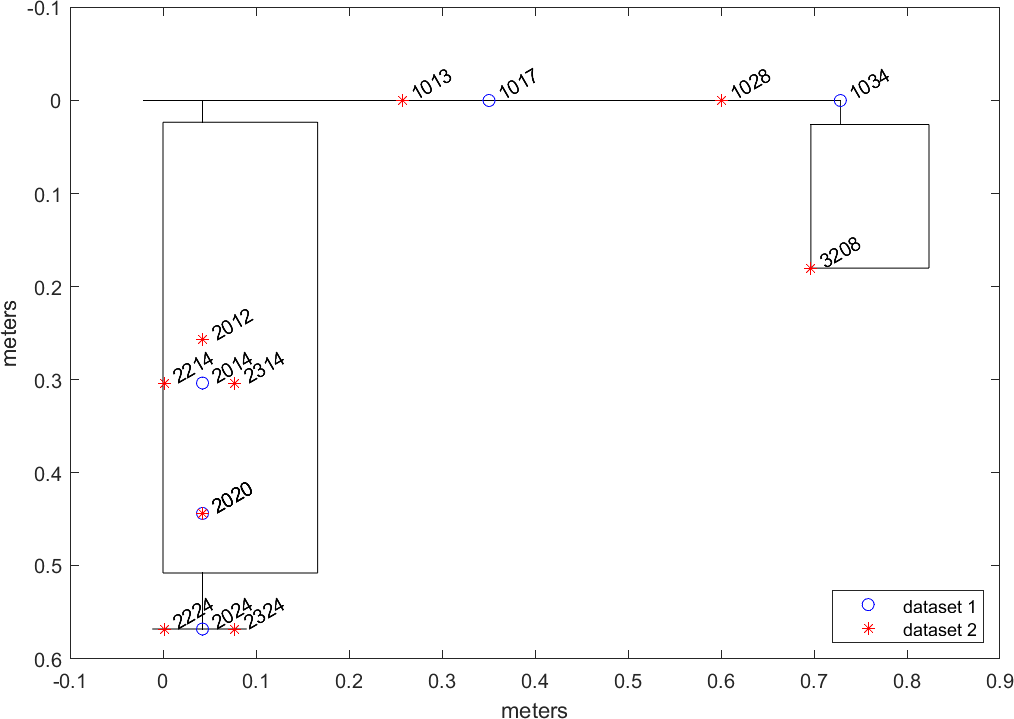
\includegraphics[width=4in]{figs/GVT/accelLocPlot.png}
    \caption{Accelerometer placement in ground vibration testing of MARGE}
    \label{fig:accelPlacement}
\end{figure}

For the second dataset, pairs of accelerometers on the wing located a short distance apart chordwise were also treated as a fictional third accelerometer by taking the difference of their signals. This was done to simulate a sensor observing only the torsional modes of the wing.

%---------------------------------------------------------------
\subsection{Test Procedure}
%---------------------------------------------------------------

Tests were performed by executing a MATLAB script which would prompt the user to name and record data. After data acquisition for a run the script automatically generated a plot of the full time-series as well as a magnified plot of the time-series data around the moment of impact. This magnified view was used to inspect for double hits from the impact hammer. The script also automatically rejected data which was of insufficient length or which had too weak or strong of an impact from the hammer.

After accelerometers were mounted to MARGE and the DAQ was connected to the host computer, the following procedure was used for each run of GVT:
\begin{enumerate}
	\item Start recording data
	\item Hit the target point with the impact hammer
	\item After at least five seconds has elapsed, stop recording data
	\item Inspect the automatically-generated plot of the time-series data for irregularities, especially double-hits of the impact hammer or bumps of the accelerometers
	\item Name and save the data
\end{enumerate}
The result of this procedure is one run of time-series data such as that shown in Figure \ref{fig:gvtTimeExample}
\begin{figure}[H]
	\centering
	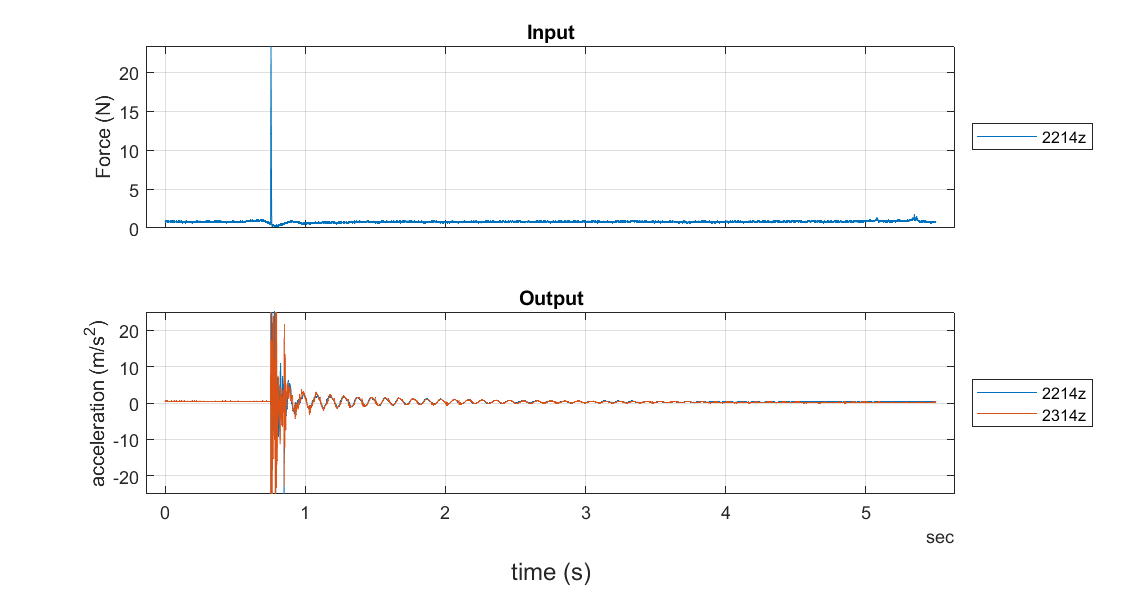
\includegraphics[width=6in]{figs/sampleGVT.png}
	\caption{Example GVT time-series data from an impulse at the location 2214z}
	\label{fig:gvtTimeExample}
\end{figure}

%%%%%%%%%%%%%%%%%%%%%%%%%%%%%%%%%%%%%%%%%%%%%%%%%%%%%%%%%%%%%%%%
\section{Generating Frequency Response Functions} %%%%%%%%%%%%%%
%%%%%%%%%%%%%%%%%%%%%%%%%%%%%%%%%%%%%%%%%%%%%%%%%%%%%%%%%%%%%%%%
\label{sec:generateFRF}

Each GVT test point (input-output combination) was post-processed to generate the frequency response functions (FRFs) of the accelerometers to the impacts. This section describes the steps in this process.

%---------------------------------------------------------------
\subsection{Time-Domain Post-Processing}
%---------------------------------------------------------------

The time-series data was truncated to to start just before the impulse input and end after $t$ seconds where $t$ was chosen to be at least four times the period of the lowest frequency of interest. (In most cases, $t=4$ seconds.) This ensured that irrelevant segments of the signal were eliminated while keeping still enough data to perform the frequency-domain analysis.

Each test point was recorded as three (in the second dataset) or five (in the first dataset) separate impacts. After truncation, the signals from these impacts were concatenated to form one continuous time-domain signal. The mean of this combined signal was then subtracted from it so that there would be no steady-state component before proceeding to compute the frequency response.

%---------------------------------------------------------------
\subsection{Computing Frequency Response Functions}
%---------------------------------------------------------------

The frequency response functions for each of these concatenated SISO signal pairs were computed using the method described in \cite{Tischler2012}. This section summarizes this method as it was implemented for the GVT data.

First, the signal was buffered into overlapping Hann windows and transformed using a chirp z-transform (CZT). The CZT has an advantage over the similar Discrete Fourier Transform (DFT) in that it has the ability to allocate the full frequency-domain resolution to the bandwidth of interest. The purpose of first buffering the signal is to reduce the effect of noise at the expense of frequency resolution.

The products of the CZT are the power spectra of the signals. For any given accelerometer power spectrum $S_y(\omega)$ and impact hammer power spectrum $S_x(\omega)$, the cross-spectrum correlation estimates can be computed as
\begin{align}
    G_{xy}(\omega) &= S_x^* \cdot S_y(\omega) \\
    G_{yx}(\omega) &= S_y^* \cdot S_x(\omega)
\end{align}
and the autospectrum correlation estimates can be computed as
\begin{align}
    G_{xx}(\omega) &= |S_x|^2	 \\
    G_{yy}(\omega) &= |S_y|^2
\end{align}

Three possible ways to estimate the FRF from the above are the $H_1$ FRF, the $H_2$ FRF, and the $H_v$ FRF:
\begin{align}
    FRF_{H_1}(\omega) &= \frac{G_{xy}(\omega)}{G_{xx}(\omega)} \\
    FRF_{H_2}(\omega) &= \frac{G_{yy}(\omega)}{G_{yx}(\omega)} \\
    \label{eq:frf}
    FRF_{H_v}(\omega) &= \sqrt{FRF_{H_1}(\omega) \cdot FRF_{H_2}(\omega)}
\end{align}
The $H_1$ estimate tends to underestimate the FRF when there is noise in the input, while the $H_2$ estimate tends to overestimate the FRF when there is noise at the output \cite{Tischler2012}. The $H_v$ estimate of the FRF is thus used in this study as a conservative choice which makes no assumption of the source or nature of noise in the system. (Subsequent references to the FRF can be assumed to refer to the $H_v$ FRF.)

The coherence can also be computed as
\begin{align}
    \operatorname{coh}(\omega) &= \frac{|G_{xy}|^2}{|G_{xx}||G_{yy}|}
    % (abs(Gxy_hat).^2)./(abs(Gxx_hat).*abs(Gyy_hat))
\end{align}
The result of this procedure is a frequency response such as that shown in Figure \ref{fig:gvtFreqExample}
\begin{figure}[H]
	\centering
	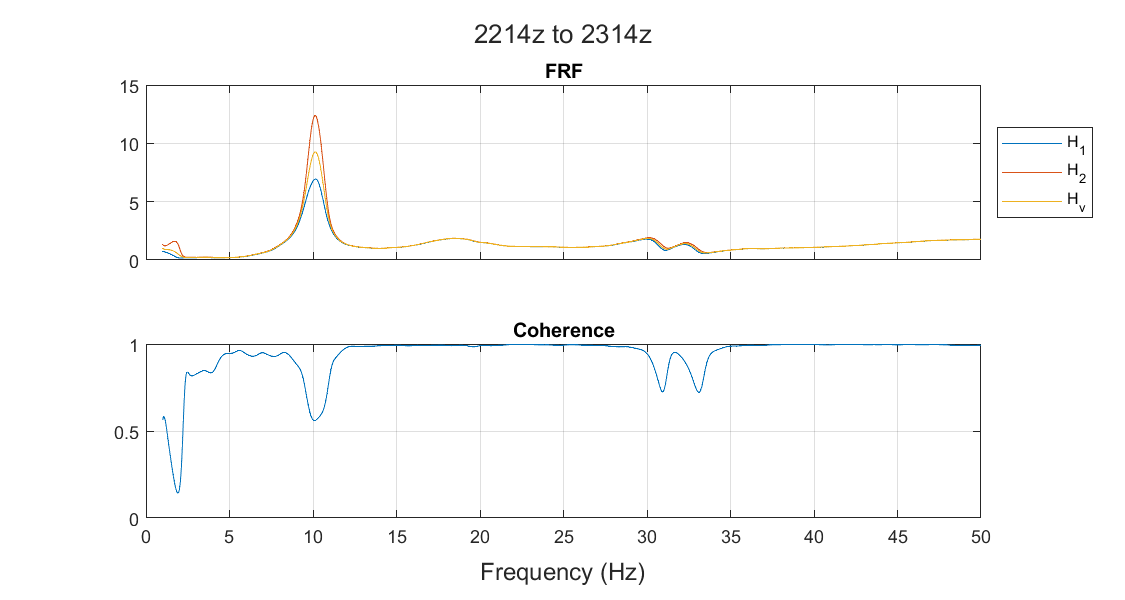
\includegraphics[width=6in]{figs/sampleGVT_FRF.png}
	\caption{Example GVT frequency response data from an impulse at the location 2214z to an accelerometer at the location 2314z}
	\label{fig:gvtFreqExample}
\end{figure}

The frequency response functions and coherence computed for the GVT data are shown in Appendix \ref{ap:frfPlots}.

%%%%%%%%%%%%%%%%%%%%%%%%%%%%%%%%%%%%%%%%%%%%%%%%%%%%%%%%%%%%%%%%
\section{Determining Modal Properties} %%%%%%%%%%%%%%%%%%%%%%%%%
%%%%%%%%%%%%%%%%%%%%%%%%%%%%%%%%%%%%%%%%%%%%%%%%%%%%%%%%%%%%%%%%

Once the FRFs were obtained, the frequencies and damping ratios of the natural modes were computed from the FRFs. This section describes this computation.

%---------------------------------------------------------------
\subsection{Computing Natural Frequencies}
%---------------------------------------------------------------

First, natural frequencies visible as peaks in the data were noted. These often were visible across multiple FRFs, confirming that they were not artifacts from the noise of a single experimental trial.

These experimental natural frequencies were compared to those predicted by the NASTRAN finite-element model; if they matched well, it was assumed that the experimental natural frequency corresponded to the mode shape generated by the NASTRAN model. This could be further validated by observing the antinodal points of the relevant NASTRAN mode shape and checking that the FRFs in which the natural frequency peaks are visible correspond to sensors placed near those antinodal points.

In some cases, there were clear natural modes visible in the experimental data that were not predicted by the NASTRAN finite-element model. It was inferred that two of these natural modes appeared in that these were torsional modes of the wing, because the FRFs they appeared most prominently in were from the aforementioned ``fictional'' accelerometers which had manipulated signals to enhance the response to torsional modes. These torsional modes were not predicted by the preliminary NASTRAN finite-element model; this was corrected in the subsequent FEM tuning process.

Each experimental natural frequency $\omega_n$ was then measured in an automated way: first, all FRFs with a local maximum magnitude at $\omega_n$ which was at least twice the magnitude of its surroundings was identified. The median of all of these measured natural frequencies, each from a different FRF, was then taken to be the true experimental natural frequency for that natural mode.

%---------------------------------------------------------------
\subsection{Computing Damping Ratios}
%---------------------------------------------------------------

The damping ratio was also measured in a similar automated way. The damping ratio was computed for each identifiable natural frequency in each FRF using the half-power method:
\begin{align}
	\zeta &= \frac{\omega_2 - \omega_1}{2\omega_n}
\end{align}
where
\begin{equation}
\begin{gathered}
	FRF(\omega_1) = FRF(\omega_2) = \frac{1}{2} FRF(\omega_n) \\
	\omega_1 < \omega_2
\end{gathered}
\end{equation}
The median of all of these damping ratios, each from a different FRF, was then taken to be the true damping ratio for that natural mode. The experimentally obtained natural frequencies and corresponding damping ratios can be found in Table \ref{tab:expModalData}.

%%%%%%%%%%%%%%%%%%%%%%%%%%%%%%%%%%%%%%%%%%%%%%%%%%%%%%%%%%%%%%%%
\section{Finite Element Model Correction} %%%%%%%%%%%%%%%%%%%%%%
%%%%%%%%%%%%%%%%%%%%%%%%%%%%%%%%%%%%%%%%%%%%%%%%%%%%%%%%%%%%%%%%
\label{sec:femCorrection}

The finite-element model was adjusted to better match the experimental GVT data as well as static testing data from a separate study. This was done by adjusting the bending and torsional stiffness of the various materials until the natural frequencies best matched that of the experiment; the values of these before and after correction are shown in Table \ref{tab:gvtAdjust}. The uncorrected and corrected natural frequencies of the FEM are compared to the experimental natural frequencies in Fig. \ref{fig:gvtAdjust}. Note that damping ratios are not involved here, as the FEM does not model damping. The damping ratios are used only in the modeling in Chapter \ref{ch:sysModeling}.

\begin{table}[h]
    \centering
    \caption{Finite-Element Model Material Parameter Adjustment}
    \label{tab:gvtAdjust}
    \begin{tabular}{ccccc}
        \hline\hline
		component & old $E$ (Pa) & old $G$ (Pa) & new $E$ (Pa) & new $G$ (Pa) \\
		\hline
		fuselage  & $2.00\times10^{11}$ & $7.58\times10^{10}$ & $1.80\times10^{11}$ & $7.60\times10^{10}$ \\ 
		wing spar & $6.89\times10^{10}$ & $2.59\times10^{10}$ & $6.89\times10^{10}$ & $1.25\times10^7$ \\
		tail spar & $6.89\times10^{10}$ & $2.59\times10^{10}$ & $6.89\times10^{10}$ & $2.59\times10^7$ \\
        \hline\hline
    \end{tabular}
\end{table}

\begin{figure}
    \centering
    \label{fig:gvtAdjust}
    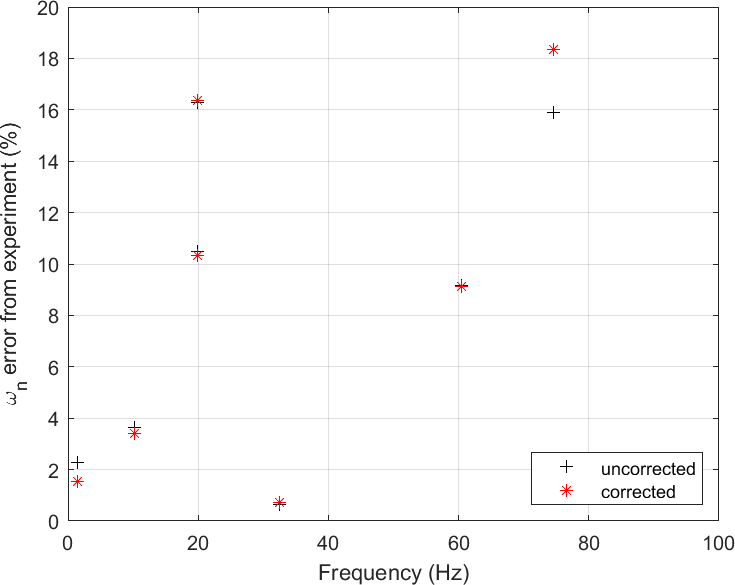
\includegraphics[width=5in]{figs/FEMcorrection.png}
    \caption{Finite-element model material parameter adjustment}
\end{figure}

\begin{table}[h]
	\centering
	\caption{Natural Frequencies of Uncorrected FEM, Corrected FEM, and Experiment}
	\label{tab:gvtCompare}
	\begin{tabular}{cccl}
		\hline\hline
		Uncorrected FEM (Hz) & Corrected FEM (Hz) & Experiment (Hz) & Description \\
		\hline
        0 & 0 &  & pitching \\
		1.454401 & 1.44397 & 1.422 & wing bending 1 \\
        10.51099 & 10.48667 & 10.142 & wing bending 2 \\
        - & 19.1997 & 18.094 & wing twisting 1 \\
        23.13519 & 21.94804 & 19.893 & fuselage in-plane bending 1 \\
        17.81394 & 16.63828 & 19.897 & fuselage bending 1 \\
        32.33148 & 32.31077 & 32.545 & wing bending 3 \\
        - & - & 51.706 & wing twisting 2 \\
        66.02579 & 66.01089 & 60.482 & wing bending 4 \\
        69.7988 & 69.29826 & & wing in-plane bending 1 \\
        62.68383 & 60.85218 & 74.521 & fuselage bending 2 \\
        113.6852 & 113.6736 & & wing bending 5 \\
        120.8188 & 120.6415 & & fuselage bending 3 \\
        161.7024 & 153.716 & & fuselage in-plane bending 2 \\
        175.9587 & 175.9407 & & wing bending 6 \\
        159.36 & 160.9085 & & fuselage bending 4 \\
        225.7709 & - & & fuselage bending 5 \\
		\hline\hline
	\end{tabular}
\end{table}